\documentclass[border=6mm]{standalone}
\usepackage{tikz}
\usepackage{fontspec}
\setmainfont{MinionPro-Regular.otf}[
  Path           = /Users/davis/Library/Fonts/,
  ItalicFont     = MinionPro-It.otf,
  BoldFont       = MinionPro-Bold.otf,
  BoldItalicFont = MinionPro-BoldIt.otf,
]
\newfontfamily\sansfont{AcuminPro-Regular.otf}[
  Path           = /Users/davis/Library/Fonts/,
  ItalicFont     = AcuminPro-Regular.otf,
  BoldFont       = AcuminPro-Semibold.otf,
  BoldItalicFont = AcuminPro-Semibold.otf,
]

\definecolor{strong}{HTML}{1A202C}
\definecolor{muted}{HTML}{718096}
\definecolor{fdrA}{HTML}{1A365D}   % FDR < 0.015 — dark
\definecolor{fdrB}{HTML}{3182CE}   % FDR 0.015–0.025
\definecolor{fdrC}{HTML}{90CDF4}   % FDR 0.025–0.05
\definecolor{bg}{HTML}{FAFAFA}
\definecolor{grid}{HTML}{EDF2F7}

\begin{document}
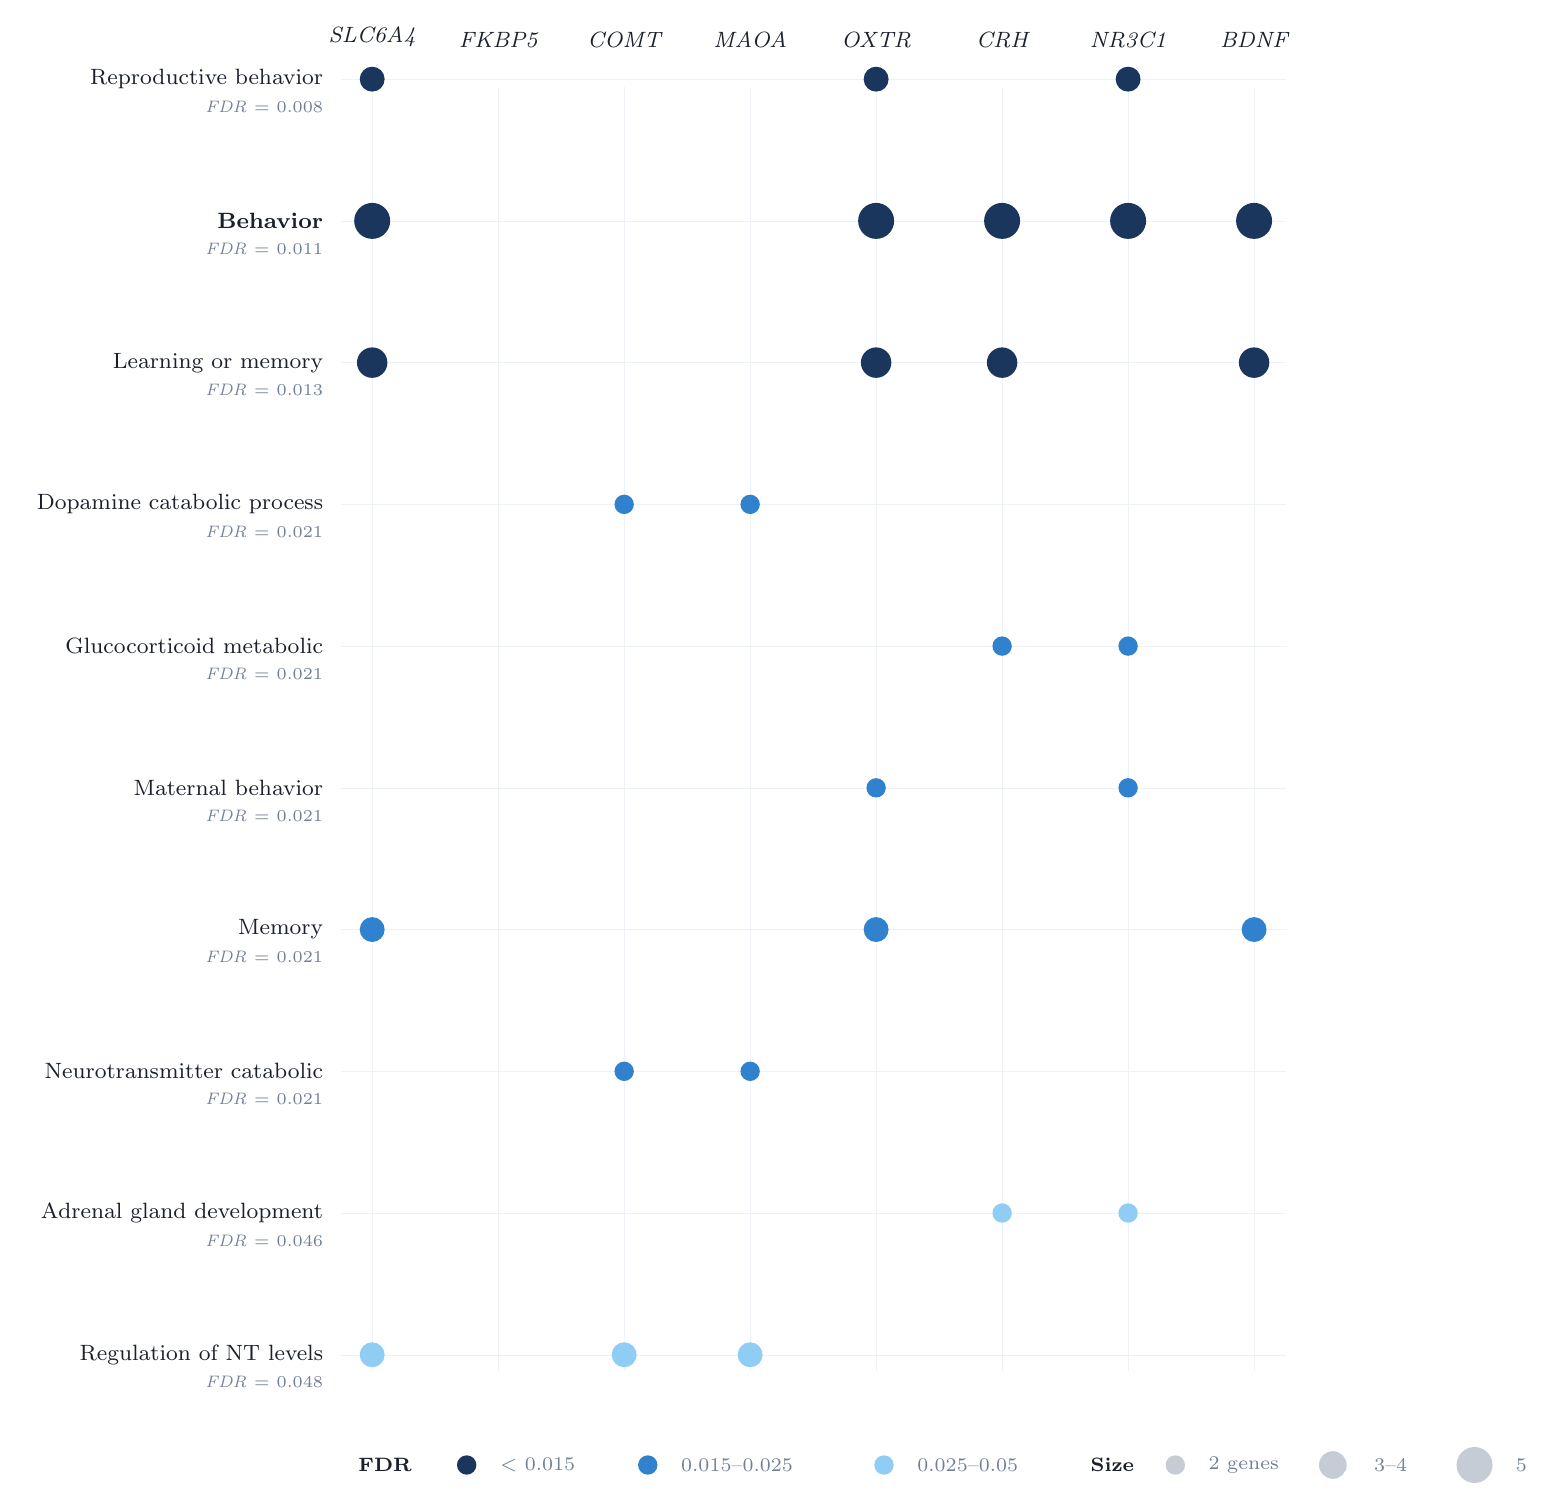
\begin{tikzpicture}[every node/.style={font=\sansfont}]

% ── Layout constants ──
% 8 gene columns, 1.6cm apart = 11.2cm data width
% 10 rows, 1.3cm apart = 11.7cm data height
\def\cw{1.6}  % column width
\def\rh{1.8}  % row height — generous vertical spacing

% ── Column x-positions (genes) ──
\foreach \i/\gene in {
  0/SLC6A4, 1/FKBP5, 2/COMT, 3/MAOA, 4/OXTR, 5/CRH, 6/NR3C1, 7/BDNF}
{
  \pgfmathsetmacro{\x}{\i*\cw}
  % Column header — horizontal, 8pt, italic gene names
  \node[font=\sansfont\fontsize{8}{10}\selectfont\itshape, color=strong,
        anchor=south, inner sep=0pt] at (\x,0.4) {\gene};
  % Thin vertical grid line
  \draw[grid, line width=0.15pt] (\x,-0.1) -- (\x,-9*\rh-0.2);
}

% ── Row data: {row index}{GO term}{FDR text}{FDR color}{dot columns (0-indexed)} ──
% Row 0 = top

% Reproductive behavior  FDR=0.008  genes: SLC6A4(0), OXTR(4), NR3C1(6)
\pgfmathsetmacro{\y}{-0*\rh}
\node[font=\sansfont\fontsize{8}{10}\selectfont, color=strong, anchor=east]
  at (-0.5,\y) {Reproductive behavior};
\node[font=\sansfont\fontsize{6.5}{8}\selectfont, color=muted, anchor=east]
  at (-0.5,\y-0.35) {\textit{FDR} = 0.008};
\draw[grid, line width=0.15pt] (-0.4,\y) -- (7*\cw+0.4,\y);
\fill[fdrA] (0*\cw,\y) circle (4.5pt);
\fill[fdrA] (4*\cw,\y) circle (4.5pt);
\fill[fdrA] (6*\cw,\y) circle (4.5pt);

% Behavior  FDR=0.011  genes: SLC6A4(0), OXTR(4), CRH(5), NR3C1(6), BDNF(7)
\pgfmathsetmacro{\y}{-1*\rh}
\node[font=\sansfont\fontsize{8}{10}\selectfont\bfseries, color=strong, anchor=east]
  at (-0.5,\y) {Behavior};
\node[font=\sansfont\fontsize{6.5}{8}\selectfont, color=muted, anchor=east]
  at (-0.5,\y-0.35) {\textit{FDR} = 0.011};
\draw[grid, line width=0.15pt] (-0.4,\y) -- (7*\cw+0.4,\y);
\fill[fdrA] (0*\cw,\y) circle (6.5pt);
\fill[fdrA] (4*\cw,\y) circle (6.5pt);
\fill[fdrA] (5*\cw,\y) circle (6.5pt);
\fill[fdrA] (6*\cw,\y) circle (6.5pt);
\fill[fdrA] (7*\cw,\y) circle (6.5pt);

% Learning or memory  FDR=0.013  genes: SLC6A4(0), OXTR(4), CRH(5), BDNF(7)
\pgfmathsetmacro{\y}{-2*\rh}
\node[font=\sansfont\fontsize{8}{10}\selectfont, color=strong, anchor=east]
  at (-0.5,\y) {Learning or memory};
\node[font=\sansfont\fontsize{6.5}{8}\selectfont, color=muted, anchor=east]
  at (-0.5,\y-0.35) {\textit{FDR} = 0.013};
\draw[grid, line width=0.15pt] (-0.4,\y) -- (7*\cw+0.4,\y);
\fill[fdrA] (0*\cw,\y) circle (5.5pt);
\fill[fdrA] (4*\cw,\y) circle (5.5pt);
\fill[fdrA] (5*\cw,\y) circle (5.5pt);
\fill[fdrA] (7*\cw,\y) circle (5.5pt);

% Dopamine catabolic process  FDR=0.021  genes: COMT(2), MAOA(3)
\pgfmathsetmacro{\y}{-3*\rh}
\node[font=\sansfont\fontsize{8}{10}\selectfont, color=strong, anchor=east]
  at (-0.5,\y) {Dopamine catabolic process};
\node[font=\sansfont\fontsize{6.5}{8}\selectfont, color=muted, anchor=east]
  at (-0.5,\y-0.35) {\textit{FDR} = 0.021};
\draw[grid, line width=0.15pt] (-0.4,\y) -- (7*\cw+0.4,\y);
\fill[fdrB] (2*\cw,\y) circle (3.5pt);
\fill[fdrB] (3*\cw,\y) circle (3.5pt);

% Glucocorticoid metabolic  FDR=0.021  genes: CRH(5), NR3C1(6)
\pgfmathsetmacro{\y}{-4*\rh}
\node[font=\sansfont\fontsize{8}{10}\selectfont, color=strong, anchor=east]
  at (-0.5,\y) {Glucocorticoid metabolic};
\node[font=\sansfont\fontsize{6.5}{8}\selectfont, color=muted, anchor=east]
  at (-0.5,\y-0.35) {\textit{FDR} = 0.021};
\draw[grid, line width=0.15pt] (-0.4,\y) -- (7*\cw+0.4,\y);
\fill[fdrB] (5*\cw,\y) circle (3.5pt);
\fill[fdrB] (6*\cw,\y) circle (3.5pt);

% Maternal behavior  FDR=0.021  genes: OXTR(4), NR3C1(6)
\pgfmathsetmacro{\y}{-5*\rh}
\node[font=\sansfont\fontsize{8}{10}\selectfont, color=strong, anchor=east]
  at (-0.5,\y) {Maternal behavior};
\node[font=\sansfont\fontsize{6.5}{8}\selectfont, color=muted, anchor=east]
  at (-0.5,\y-0.35) {\textit{FDR} = 0.021};
\draw[grid, line width=0.15pt] (-0.4,\y) -- (7*\cw+0.4,\y);
\fill[fdrB] (4*\cw,\y) circle (3.5pt);
\fill[fdrB] (6*\cw,\y) circle (3.5pt);

% Memory  FDR=0.021  genes: SLC6A4(0), OXTR(4), BDNF(7)
\pgfmathsetmacro{\y}{-6*\rh}
\node[font=\sansfont\fontsize{8}{10}\selectfont, color=strong, anchor=east]
  at (-0.5,\y) {Memory};
\node[font=\sansfont\fontsize{6.5}{8}\selectfont, color=muted, anchor=east]
  at (-0.5,\y-0.35) {\textit{FDR} = 0.021};
\draw[grid, line width=0.15pt] (-0.4,\y) -- (7*\cw+0.4,\y);
\fill[fdrB] (0*\cw,\y) circle (4.5pt);
\fill[fdrB] (4*\cw,\y) circle (4.5pt);
\fill[fdrB] (7*\cw,\y) circle (4.5pt);

% Neurotransmitter catabolic  FDR=0.021  genes: COMT(2), MAOA(3)
\pgfmathsetmacro{\y}{-7*\rh}
\node[font=\sansfont\fontsize{8}{10}\selectfont, color=strong, anchor=east]
  at (-0.5,\y) {Neurotransmitter catabolic};
\node[font=\sansfont\fontsize{6.5}{8}\selectfont, color=muted, anchor=east]
  at (-0.5,\y-0.35) {\textit{FDR} = 0.021};
\draw[grid, line width=0.15pt] (-0.4,\y) -- (7*\cw+0.4,\y);
\fill[fdrB] (2*\cw,\y) circle (3.5pt);
\fill[fdrB] (3*\cw,\y) circle (3.5pt);

% Adrenal gland development  FDR=0.046  genes: CRH(5), NR3C1(6)
\pgfmathsetmacro{\y}{-8*\rh}
\node[font=\sansfont\fontsize{8}{10}\selectfont, color=strong, anchor=east]
  at (-0.5,\y) {Adrenal gland development};
\node[font=\sansfont\fontsize{6.5}{8}\selectfont, color=muted, anchor=east]
  at (-0.5,\y-0.35) {\textit{FDR} = 0.046};
\draw[grid, line width=0.15pt] (-0.4,\y) -- (7*\cw+0.4,\y);
\fill[fdrC] (5*\cw,\y) circle (3.5pt);
\fill[fdrC] (6*\cw,\y) circle (3.5pt);

% Regulation of NT levels  FDR=0.048  genes: SLC6A4(0), COMT(2), MAOA(3)
\pgfmathsetmacro{\y}{-9*\rh}
\node[font=\sansfont\fontsize{8}{10}\selectfont, color=strong, anchor=east]
  at (-0.5,\y) {Regulation of NT levels};
\node[font=\sansfont\fontsize{6.5}{8}\selectfont, color=muted, anchor=east]
  at (-0.5,\y-0.35) {\textit{FDR} = 0.048};
\draw[grid, line width=0.15pt] (-0.4,\y) -- (7*\cw+0.4,\y);
\fill[fdrC] (0*\cw,\y) circle (4.5pt);
\fill[fdrC] (2*\cw,\y) circle (4.5pt);
\fill[fdrC] (3*\cw,\y) circle (4.5pt);

% ── Legend ──
\pgfmathsetmacro{\ly}{-9*\rh - 1.4}

\node[font=\sansfont\fontsize{7}{9}\selectfont\bfseries, color=strong,
      anchor=west] at (-0.3,\ly) {FDR};
\fill[fdrA] (1.2,\ly) circle (3.5pt);
\node[font=\sansfont\fontsize{7}{9}\selectfont, color=muted, anchor=west]
  at (1.5,\ly) {$<$ 0.015};
\fill[fdrB] (3.5,\ly) circle (3.5pt);
\node[font=\sansfont\fontsize{7}{9}\selectfont, color=muted, anchor=west]
  at (3.8,\ly) {0.015--0.025};
\fill[fdrC] (6.5,\ly) circle (3.5pt);
\node[font=\sansfont\fontsize{7}{9}\selectfont, color=muted, anchor=west]
  at (6.8,\ly) {0.025--0.05};

\node[font=\sansfont\fontsize{7}{9}\selectfont\bfseries, color=strong,
      anchor=west] at (9,\ly) {Size};
\fill[muted!40] (10.2,\ly) circle (3.5pt);
\node[font=\sansfont\fontsize{7}{9}\selectfont, color=muted, anchor=west]
  at (10.5,\ly) {2 genes};
\fill[muted!40] (12.2,\ly) circle (5pt);
\node[font=\sansfont\fontsize{7}{9}\selectfont, color=muted, anchor=west]
  at (12.6,\ly) {3--4};
\fill[muted!40] (14,\ly) circle (6.5pt);
\node[font=\sansfont\fontsize{7}{9}\selectfont, color=muted, anchor=west]
  at (14.4,\ly) {5};

\end{tikzpicture}
\end{document}
